\section{Zusammenhänge von Auslastungs- und Potentialspielen}\label{sec:Auslastungsspiele}

\todo[inline]{Welche Endlichkeitsvoraussetzungen benötigt man hier jeweils?}

In \cite{RosenthalPotential} führte \citeauthor{RosenthalPotential} Auslastungsspiele als Klasse von Spielen ein, welche immer ein exaktes Potential (und damit ein Nash-Gleichgewicht) besitzen. Später zeigten \citeauthor{MonShap} in \cite[Theorem 3.2]{MonShap}, dass diese Klasse bis auf (kostenerhaltende) Isomorphie bereits \emph{alle} Spiele mit exaktem Potential umfasst. Zusammengefasst gilt also:

\begin{satz}\label{satz:MondererShapley}
	Jedes $N$-Personen-Auslastungsspiel besitzt ein exaktes Potential und jedes exakte $N$-Personen-Potentialspiel ist äquivalent zu einem Auslastungsspiel.
\end{satz}

\begin{proof}
	Sei $\Gamma(M)$ ein beliebiges Auslastungsspiel. Dann definieren wir wie folgt die Rosenthal-Potentialfunktion:
		\[P: S \to \IR: s \mapsto \sum_{r \in R}\sum_{k=1}^{l_r(s)} g_r(k) \]
	Die Funktion ist wohldefiniert, da die insgesamt $N$ Spieler zusammen nur endlich viele Ressourcen nutzen können und daher beide Summen endlich sind. Sie ist ferner ein exaktes Potential, denn zu einem Strategieprofil $s \in S$ und einer weiteren Strategie $\hat{s}_i$ von Spieler $i$ gilt:
	\begin{align*}
		P(s) 	&- P(s\mid \hat{s}_i) = \sum_{r \in R}\sum_{k=1}^{l_r(s)} g_r(k) - \sum_{r \in R}\sum_{k=1}^{l_r(s\mid \hat{s}_i)} g_r(k) = \sum_{r \in s_i \setminus \hat{s}_i} g_r(l_r(s)) - \sum_{r \in \hat{s}_i \setminus s_i} g_r(l_r(s)+1) = \\
				&= \sum_{r \in s_i \setminus \hat{s}_i} g_r(l_r(s)) + \sum_{r \in s_i \cap \hat{s}_i} g_r(l_r(s)) - \sum_{r \in s_i \cap \hat{s}_i} g_r(l_r(s \mid \hat{s}_i)) - \sum_{r \in \hat{s}_i \setminus s_i} g_r(l_r(s\mid \hat{s}_i)) = \\
				&= \sum_{r \in s_i} g_r(l_r(s)) - \sum_{r \in \hat{s}_i} g_r(l_r(s\mid \hat{s}_i)) = c_i(s) - c_i(s \mid \hat{s}_i)
	\end{align*}
	
		
	Für die umgekehrte Richtung orientieren wir uns an dem Beweis in \cite[Theorem 1]{MultiPotGames}. Gegeben also ein Spiel $\Gamma = (I, X, (c_i)_{i\in i})$ mit einem exakten Potential $P$. Hierzu definieren wir folgendes Auslastungsmodell $M = (I, R, (S_i)_{i \in I}, (g_r)_{r \in R})$:
	\begin{itemize}
		\item $R \coloneqq R_K \cup R_D \subseteq \prod_{i \in I}\Pc(X_i)$, wobei $R_K \coloneqq \Set{\left(\{x_i\}\right)_{i \in I} | x_i \in X_i }$ und \\ $R_D \coloneqq \Set{(Y_i)_{i \in I} | \exists \hat{i} \in I: Y_{\hat{i}} = X_{\hat{i}}, \forall i \neq \hat{i}: \abs{X_i \setminus Y_i} = 1 }$.
		\item \[g_r(k) \coloneqq 
					\begin{cases}
						P(x), 					&r = \left(\{x_i\}\right)_{i \in I} \in R_k 													\text{ und } k=N \\
						c_{\hat{i}}(x) - P(x), 	&r = \left(X_i\setminus\{x_i\}\right)_{i \in I\setminus\hat{i}} \times X_{\hat{i}} \in R_D 	\text{ und } k=1 \\
						0,						&\text{sonst}
					\end{cases}\]
				\todo[inline]{Wohldefiniertheit!}
		\item $S_i \coloneqq \Set{ \Set{r \in R | x_i \in r_i} | x_i \in X_i }$
	\end{itemize}
	Die induzierten Lastfunktionen sind automatisch wohldefiniert, da die Spielermenge endlich ist, die Wohldefiniertheit der Kostenfunktionen $d_i$ folgt dann aus dem Beweis der Äquivalenz der Spiele $\Gamma$ und $\Gamma(M)$. Dazu betrachten wir den Morphismus $(\id, \phi): \Gamma \to \Gamma(M)$, wobei $\phi_i(x) \coloneqq s(x_i) \coloneqq \{r \in R \mid x_i \in r_i\}$.
	\begin{align*}
		d_i(\phi(x)) = \sum_{r \in \phi(x)_i} g_r(l_r(\phi(x))) = \dots
	\end{align*}\todo{Beweis vervollständigen}
\end{proof}

Auslastungsspiele sind also nicht nur \emph{ein} Beispiel für Spiele mit exaktem Potential, sondern in gewissem Sinne (nämlich bis auf Isomorphie) sogar \emph{das} Beispiel für solche Spiele. Eine naheliegende Frage ist nun, ob es ähnliche Klassen von \glqq auslastungsartigen\grqq{} Spielen gibt, welche genau den Spielen mit allgemeineren Potentialen entsprechen. Im Folgenden werden wir versuchen eine zu gewichteten Potentialspielen passende Verallgemeinerung von Auslastungsspielen zu finden.

\subsection{Von ungewichtet zu gewichtet}

\subsubsection{Gewichtete Auslastungsspiele}

Für gewichtete Auslastungsspiele zeigen \citeauthor{CharExGewPotinWCG} in \cite[Theorem 3.9]{CharExGewPotinWCG}, dass die einzigen beiden Klassen stetiger Funktionen, die (als Kostenfunktionen verwendet) ausschließlich Spiele mit gewichtetem Potential erzeugen, affin lineare Funktionen bzw. exponentielle Funktionen (mit gemeinsamem Exponenten) sind:

\begin{satz}\label{satz:CharExGewPotinWCG}
	Gegeben eine Menge von stetigen Funktionen $C$. Dann besitzt genau dann jedes gewichtete Auslastungsspiel, welches nur Funktionen aus $C$ als Kostenfunktionen verwendet, ein gewichtetes Potential, wenn $C$
	\begin{itemize}
		\item entweder ausschließlich affin lineare Funktionen enthält\todo{Fälle: Exaktes Potential/gewichtetes Potential unterscheiden}
		\item oder ausschließlich Funktionen der Form $c(l) = a_c\cdot b^l + d_c$ enthält.
	\end{itemize}
\end{satz}

In \cite[Theorem 5.1]{CharExNGinWCG} zeigen \citeauthor{CharExNGinWCG} weiter, dass diese beiden Klassen von Kostenfunktionen unter allen Klassen \emph{stetiger} Funktionen gleichzeitig auch die einzigen sind, die die Existenz eines Nash-Gleichgewichtes garantieren.\footnote{zudem sind es auch noch die einzigen Klassen, welche für jedes gewichtete Auslastungsspiel das Erfüllen der FIP sicherstellen.}

Da nun für endliche Spiele alle der in \Cref{sec:Potentiale} definierten Potentiale die Existenz eines Nash-Gleichgewichtes garantieren, folgt hiermit direkt, dass es auch für die allgemeineren Potentialbegriffe keine größeren oder anderen Klassen von stetigen Funktionen gibt, die immer die Existenz eines entsprechenden Potentials sicher stellen.

Zusammen zeigen diese beiden Sätze bereits deutlich, dass der Schritt vom ungewichteten Fall zum gewichteten auf Seite der Auslastungsspiele erheblich größer ist als auf Seite der Potentiale. Tatsächlich zeigt \citeauthor{ReprOfFiniteGamesAsNCG} in \cite{ReprOfFiniteGamesAsNCG}, dass dieser Verallgemeinerungsschritt für Auslastungsspiele bereits der größtmögliche ist, denn es gilt:

\begin{satz}
	Jedes Spiel ist äquivalent zu einem gewichteten Auslastungsspiel \todo{(sogar Netzwerkauslastungsspiel mit ...)}.
\end{satz}

Die Menge der gewichteten Auslastungsspiele umfasst also (bis auf kostenerhaltende Isomorphie) bereits \emph{alle} (endlichen) Spiele in strategischer Form. Möchte man daher eine wirklich analoge Verallgemeinerung von Auslastungsspielen passend zu gewichteten Potentialspielen finden, muss man also andere Varianten betrachten Gewichte ins Spiel zu bringen. In \Cref{def:gewAuslastungsspiel} hatten wir bereits zwei solche gesehen, welche wir nun näher untersuchen wollen:

\subsubsection{Lastgewichtete Auslastungsspiele}

Die erste alternative Klasse von Auslastungsspielen sind die lastgewichteten Auslastungsspiele. \citeauthor{CharExGewPotinWCG} beobachten in \cite{CharExGewPotinWCG}, dass lastgewichtete Auslastungsspiele (die dort als normalisierte Auslastungsspiele bezeichnet werden) zwar nicht äquivalent, aber doch unter verschiedenen Aspekten sehr ähnlich zu allgemeinen gewichteten Auslastungsspielen sind. Dieser Zusammenhang lässt sich nun leicht durch einen passenden Isomorphiebegriff formalisieren - es gilt nämlich:

\begin{lemma}
	Jedes lastgewichtete Auslastungsspiel ist gewichtet isomorph zu einem gewichteten Auslastungsspiel und umgekehrt. Die beiden Spiele basieren dabei jeweils auf dem gleichen Auslastungsmodell.
\end{lemma}

\begin{proof}
	Der Existenz eines solchen Isomorphismus folgt direkt aus der auch in \cite{CharExGewPotinWCG} gemachten Beobachtung ...
\end{proof}

Hieraus ergeben sich dann direkt die in \cite{CharExGewPotinWCG} beobachteten Zusammenhänge zwischen gewichteten und lastgewichteten Auslastungsspielen:

\begin{kor}.
	
	\todo[inline]{Beobachtungen}
\end{kor}

Insbesondere sehen wir damit aber auch, dass lastgewichtete Auslastungsspiele ebenfalls eine zu starke Verallgemeinerung von ungewichteten Auslastungsspielen sind, um eine Entsprechung der gewichteten Potentialspiele sein zu können.


\subsubsection{Kostengewichtete Auslastungsspiele}

Wie sich herausstellt sind kostengewichtete Auslastungsspiele hingegen ein geeigneter Kandidat:

\begin{satz}
	Jedes kostengewichtete Auslastungsspiel besitzt ein gewichtetes Potential und jedes Spiel mit einem gewichteten Potential ist äquivalent zu einem kostengewichteten Auslastungsspiel.
\end{satz}

Nicht nur entspricht dieser Satz genau dem von \citeauthor{MonShap} bewiesenen Satz für ungewichtete Auslastungsspiele und exakte Potentiale (\Cref{satz:MondererShapley}), auch der Beweis erfolgt völlig analog. 

\begin{proof}
	Sei $\Gamma$ ein kostengewichtetes Auslastungsspiel mit Gewichtsvektor $w := (w_i)_{i\in I}$. Dann ist die Rosenthal-Potentialfunktion (vgl. \cite{RosenthalPotential}) $P(x) := \sum_{r \in R}\sum_{k=1}^{l_r(x)}g_r(k)$ ein $w$-Potential für $\Gamma$, denn es gilt:
	
		\todo[inline]{Beweis!}	
		
	Ist umgekehrt $\Gamma$ ein Spiel mit einem gewichteten Potential $P$ (mit Gewichtsvektor $w$), so definieren wir wie folgt ein kostengewichtetes Auslastungsspiel (wir folgen hier dem Beweis in \cite[Theorem 1]{MultiPotGames}):
	
		\todo[inline]{Definition kostengewichtetes Auslastungsspiel}
	
	Zum Beweis der Äquivalenz der beiden Spiele betrachte man folgenden kostenerhaltenden Isomorphismus:
	
		\todo[inline]{Definition Iso}
\end{proof}

Zusammen mit \Cref{satz:CharExGewPotinWCG} wissen wir nun ...

\todo[inline]{Direkte Konstruktion eines ungewichteten Auslastungsspiels zu gew. mit affin-linearen Kosten (wie ähnlich ist diese zu dem Beweis der Existenz eines exakten Potentials von Fotakis et al?)

Kann man irgendwas zu Spielen mit expontentiellen Kosten sagen?}


\subsection{Überblick}

\begin{figure}[h]\centering
	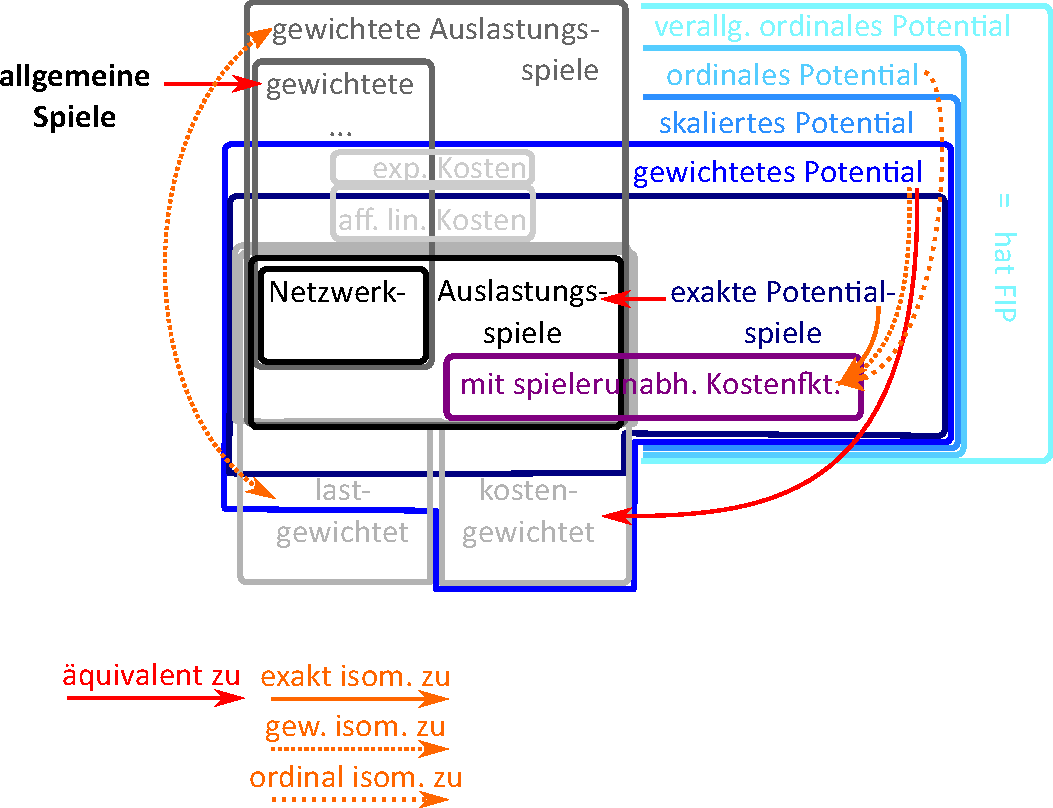
\includegraphics[width=.7\textwidth]{../Bilder/EulerDiagramm.pdf}
	\caption{Zusammenhänge zwischen den verschiedenen Spieleklassen für endliche Spiele}
\end{figure}